%!TEX root = main.tex
\section{Neutron Attenuation In Water} % (fold)
\label{sec:neutron_attenuation_in_water}


\subsection{Boron Tri-Flouride Detector} % (fold)
\label{ssub:boron_tri_flouride_detector}
The $\text{BF}_3$ detector contains a boron trifluoride gas at 0.5 to 1 atmospheres which acts as both a target for slow neutron conversion into secondary particles, as well as a proportional gas. A large potential difference is applied across the gas, the cathode held at ground is the outer tube of the detector and the anode, at the high voltage, is a single wire that passes through the centre of the detector, see figure \ref{fig:bf3detector}. When a neutron is incident in the reactor, one of the reaction below takes place.
\begin{align}
	\cf{^{10}_{5}B} + \cf{^{1}_{0}n} &\rightarrow \cf{^{7}_{3}Li} + \cf{^{4}_{2}\alpha} \label{eq:bf31}\\
	\cf{^{10}_{5}B} + \cf{^{1}_{0}n} &\rightarrow \cf{^{7}_{3}Li^*} + \cf{^{4}_{2}\alpha} \label{eq:bf32}
\end{align} 

The products of these two equations differ only by the energy of the lithium which, in some cases, is left in an excited metastable state with a slightly different energy. The relative probabilities of each reaction is 96\% for equation \ref{eq:bf31} and 4\% for equation \ref{eq:bf32}. The resulting ions that are created are attracted to the poles of the detector and so provide a voltage through it. This provides a signal which is sent to the processing computer. It should be noted that this detector cannot give any information of the energy of the neutron since the formation of the ions is independent of energy over a certain level. Instead, this detector is used simply as a counter to obtain a value for the number of neutrons hitting it in a specified time period. 

The electric field close to the wire increases quickly ($E\propto\frac{1}{r^2}$) and so a Townsend avalanche forms near to the wire when a reaction occurs. This involves the electrons being accelerated greatly by the electric field which causes the gas to conduct through the avalanche producing the signal.
\begin{figure}[ht]
	\centering
	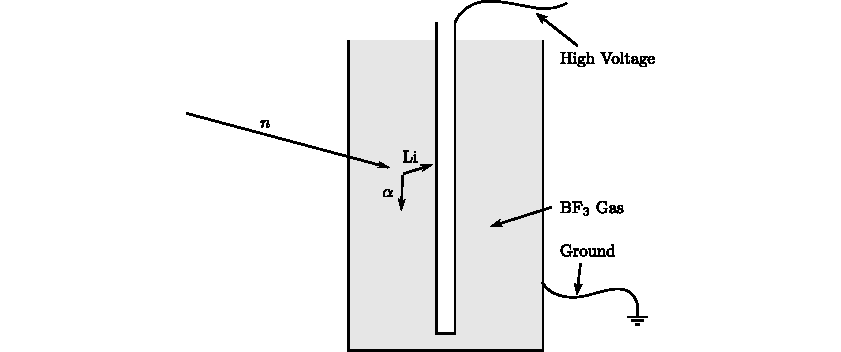
\includegraphics[width=0.9\textwidth]{BF3detector.pdf}
	\caption{The $\text{BF}_4$ detector uses a high charge to create a flow of ions to measure the incoming neutron. It cannot measure the energy, but simply gives a count for the number of neutrons incident in the detector. The anode and cathode create a large electric field inside the detector that creates the flow of charge used to count the incoming particles.\label{fig:bf3detector}}
\end{figure}

\subsubsection{Wall Effect} % (fold)
\label{ssub:wall_effect}
The BF$_3$ detector shall be used for several purposes later, so it is worth discussing some of the features of the data that is produced by this detector. Figure \ref{fig:walleffect} shows a typical spectrum from the BF$_3$ detector. This shows a main peak, a smaller, higher energy secondary peak and an example of the wall effect.
\begin{figure}[ht]
  \centering
  % \begin{overpic}[width=0.6\columnwidth,grid]{walleffect.pdf}
  \begin{overpic}[width=0.6\columnwidth]{walleffect.pdf}
    \put(20,36){Wall effect}
    \put(20,31){continuum}
    \put(30,30){\vector(-1,-4){4}}
    \put(30,30){\vector(3,-4){10}}
    \put(67,50){$\text{Li}^* + \alpha$}
    \put(80,10){$\text{Li} + \alpha$}
    \put(42,19){$\alpha$}
    \put(30,13){Li}
  \end{overpic}
  \caption{An exemplar spectrum from the BF$_3$ detector showing the wall effect when one of the products from equation \ref{eq:bf31} escapes the detector.\label{fig:walleffect}}
\end{figure}

The two steps in the count number at lower channel numbers is known as the wall effect. These are due to the detector being finite and so there is a chance that one of the products from the reaction escapes from the detector. Due to the relative masses of the particles created, $\alpha$ and Li, the $\alpha$ particle takes most of the energy from the original neutron and so when it is lost from the detector, the recoded energy is lower.

Other features of the spectrum are the abrupt cut-off at the low channel numbers. This is to reduce the background counts that are present in this region from obscuring the rest of the data. 
% subsubsection wall_effect (end)

% subsubsection boron_tri_flouride_detector (end)

% section neutron_attenuation_in_water (end)

